\documentclass[border=3pt,varwidth]{standalone}
\usepackage{amsmath,amssymb}
\usepackage{tikz}
\usetikzlibrary{arrows.meta,calc,decorations.markings,patterns,positioning,angles,quotes}
\tikzset{
  >=Stealth,
  every node/.style={font=\normalsize},
  wire/.style={line width=0.9pt},
  thinwire/.style={line width=0.6pt},
  fieldline/.style={line width=0.6pt,-{Stealth[length=2.2mm]}},
  axis/.style={line width=0.7pt,-{Stealth[length=2.2mm]}},
  dashedwire/.style={line width=0.9pt,dash pattern=on 3pt off 2pt},
  resistor/.style={line width=0.9pt},
  chargepos/.style={circle,draw,line width=0.8pt,minimum size=5mm,inner sep=0pt},
  dotcharge/.style={circle,fill,inner sep=0pt,minimum size=2.4pt}
}
% Draw a resistor box centered at (x,y) with width w, height h, horizontal
\newcommand{\resbox}[4]{%
  % #1=x #2=y #3=halfwidth #4=label
  \draw[resistor] (#1-#3,#2-0.18) rectangle (#1+#3,#2+0.18);
  \ifx\\#4\\\else\node[above=2pt] at (#1,#2+0.18) {#4};\fi
}
% Battery symbol: long thin line (+) then short thick line (-), centered at (x,y)
\newcommand{\battery}[2]{%
  % #1=x #2=y ; long line left=+, short line right=- by default orientation
  \draw[wire] (#1-0.09,#2-0.32) -- (#1-0.09,#2+0.32);
  \draw[line width=2.6pt] (#1+0.09,#2-0.16) -- (#1+0.09,#2+0.16);
}

\begin{document}
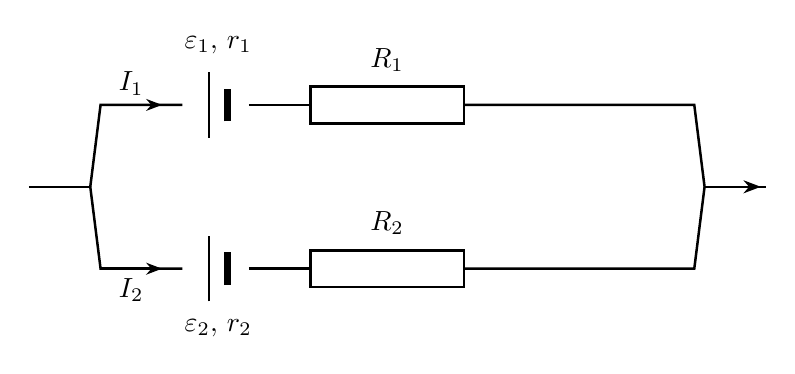
\begin{tikzpicture}[scale=1.3]
  \coordinate (L) at (-3.0,0);
  \coordinate (Rn) at (3.0,0);
  \draw[wire] (-3.6,0) -- (L);
  \draw[wire] (Rn) -- (3.6,0);
  \draw[wire,-{Stealth[length=2.2mm]}] (3.1,0) -- (3.55,0);

  \draw[wire] (L) -- (-2.9,0.8) -- (-2.1,0.8);
  \draw[wire,-{Stealth[length=2mm]}] (-2.9,0.8) -- (-2.3,0.8);
  \node[above] at (-2.6,0.8) {$I_1$};
  \battery{-1.75}{0.8}
  \node[above] at (-1.75,1.2) {$\varepsilon_1,\,r_1$};
  \draw[wire] (-1.45,0.8) -- (-0.85,0.8);
  \resbox{-0.1}{0.8}{0.75}{$R_1$}
  \draw[wire] (0.65,0.8) -- (2.9,0.8) -- (Rn);

  \draw[wire] (L) -- (-2.9,-0.8) -- (-2.1,-0.8);
  \draw[wire,-{Stealth[length=2mm]}] (-2.9,-0.8) -- (-2.3,-0.8);
  \node[below] at (-2.6,-0.8) {$I_2$};
  \battery{-1.75}{-0.8}
  \node[below] at (-1.75,-1.2) {$\varepsilon_2,\,r_2$};
  \draw[wire] (-1.45,-0.8) -- (-0.85,-0.8);
  \resbox{-0.1}{-0.8}{0.75}{$R_2$}
  \draw[wire] (0.65,-0.8) -- (2.9,-0.8) -- (Rn);
\end{tikzpicture}
\end{document}
